Au début de ce stage, le logiciel \textit{symbolist} en est déjà à un état de développement avancé. Cette section détaille l'état de l'application d'un point de vue fonctionnel, technologique et architectural, tel qu'il se trouvait au début de la période de formation.

\paragraph{Interface graphique} Au commencement du stage, l'interface graphique de \textit{symbolist} offre déjà les fonctionnalités basiques de dessin sur l'espace de la partition. Les différentes vues composants l'éditeur graphique de \textit{symbolist} sont présentées en figure \ref{fig:symbolistUIBefore}.

\begin{figure}[H]
	\centering
	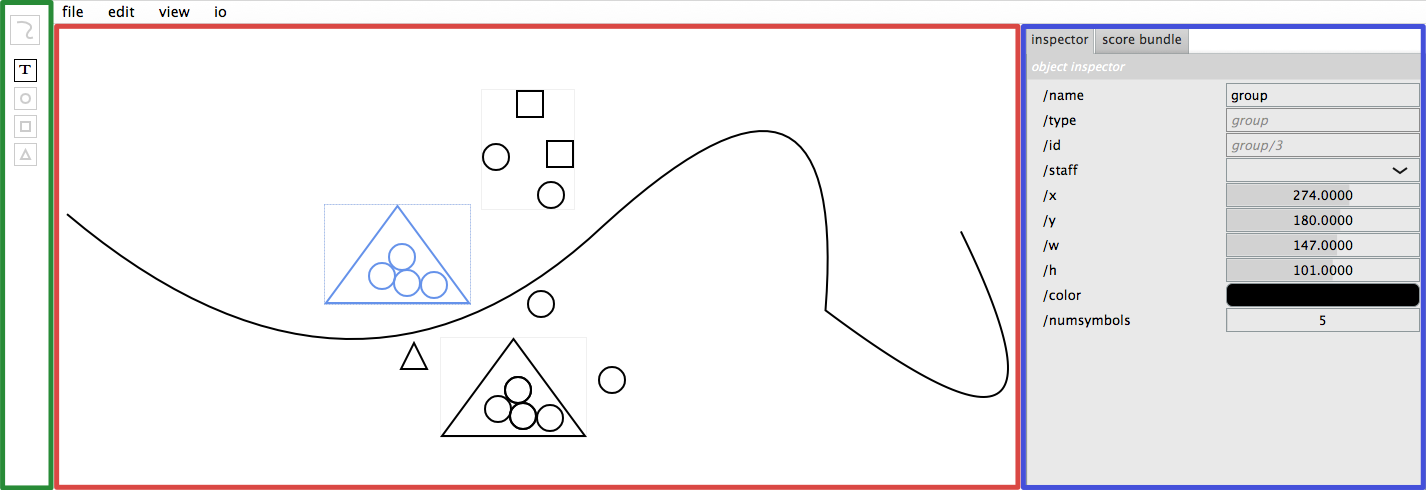
\includegraphics[keepaspectratio=true, width=\textwidth]{LeProjetSymbolist/i/symbolistUIBefore.png}
	\caption{Éditeur graphique de \textit{symbolist}}
	\label{fig:symbolistUIBefore}
	\small
	\it
	En \textcolor{green}{vert}, la palette des symboles disponibles et dessinables sur la partition. En \textcolor{red}{rouge}, la partition, ou l'espace de composition et d'édition des symboles. En \textcolor{blue}{bleu}, l'inspecteur de symboles, qui présente le bundle OSC associé au symbole graphique couramment sélectionné (symbole surligné en bleu dans la partition).
\end{figure}

L'éditeur graphique de \textit{symbolist} permet à l'utilisateur de dessiner directement sur la partition à l'aide de la souris, dans une modèle d'interaction \textit{wysiwyg} (\textit{what you see is what you get}). Dans \textit{symbolist}, la partition fait référence à l'espace graphique où les symboles sont placés et édités par l'utilisateur. 

\paragraph{Environnements d'interactions} De plus, l'éditeur graphique n'est pas le seul moyen d'interagir avec le logiciel \textit{symbolist}. En effet, \textit{symbolist} est également déployer dans une version \textit{objet} pour l'environnement \textit{Max} et l'environnement \textit{OpenMusic}. Dans ces environnements, l'application \textit{symbolist} est représentée comme une boîte, recevant et envoyant des messages à d'autres objets. Les différents messages auxquels répond l'objet \textit{symbolist} dans l'environnement Max sont présentés en figure \ref{fig:symbolistMaxObject}.

\begin{figure}[H]
	\centering
	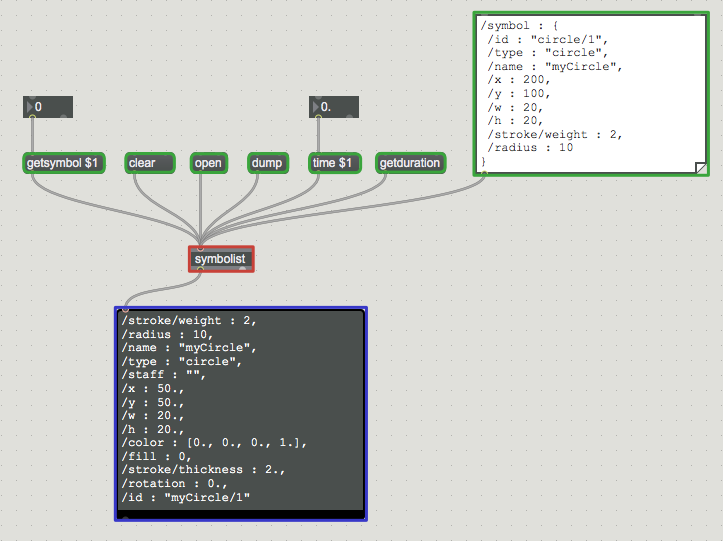
\includegraphics[keepaspectratio=true, width=0.8\textwidth]{LeProjetSymbolist/i/symbolistMaxObject.png}
	\caption{L'objet \textit{symbolist} dans Max}
	\label{fig:symbolistMaxObject}
	\small
	\it
	En \textcolor{red}{rouge}, l'objet \emph{symbolist} représenté, comme tous les objets \emph{Max}, sous forme de boîte. En \textcolor{green}{vert}, les messages pouvant être envoyés à l'objet \emph{symbolist}.
	En \textcolor{blue}{bleu}, un afficheur de bundle OSC, proposé par une librairie indépendante, témoin des messages de sortie générés par l'objet \emph{symbolist}.  
\end{figure}

Les messages\footnote{Dans Max, un message peut être envoyé à un objet via l'objet \textit{message}, qui n'est autre qu'un bouton cliquable avec un label, à connecter à l'entrée d'un receveur.} compris par l'objet \textit{symbolist} permettent de lire et d'écrire des symboles dans la partition.
Comme exemples de messages de lecture, \lstinline|getsymbol n|, lit le \textit{n-ième} symbole de la partition, \lstinline|time t|, lit le contenu de la partition au temps \textit{t}…
Le résultat de la lecture est envoyé sur la sortie de l'objet \textit{symbolist}.

L'écriture de symboles dans la partition se fait par l'envoi de bundles OSC en entrée de l'objet \textit{symbolist} (voir la figure \ref{fig:symbolistMaxObject}, en haut à droite). 
Enfin, l'éditeur graphique peut être lancé par l'envoi du message \lstinline|open|.

\textit{symbolist} est également déployé dans une version objet \textit{OpenMusic}. La figure \ref{fig:symbolistOMObject} montre un exemple de computation de partition avec l'objet \textit{symbolist} (nommé \textit{sym-score}) dans \textit{OpenMusic}.

\begin{figure}[H]
	\centering
	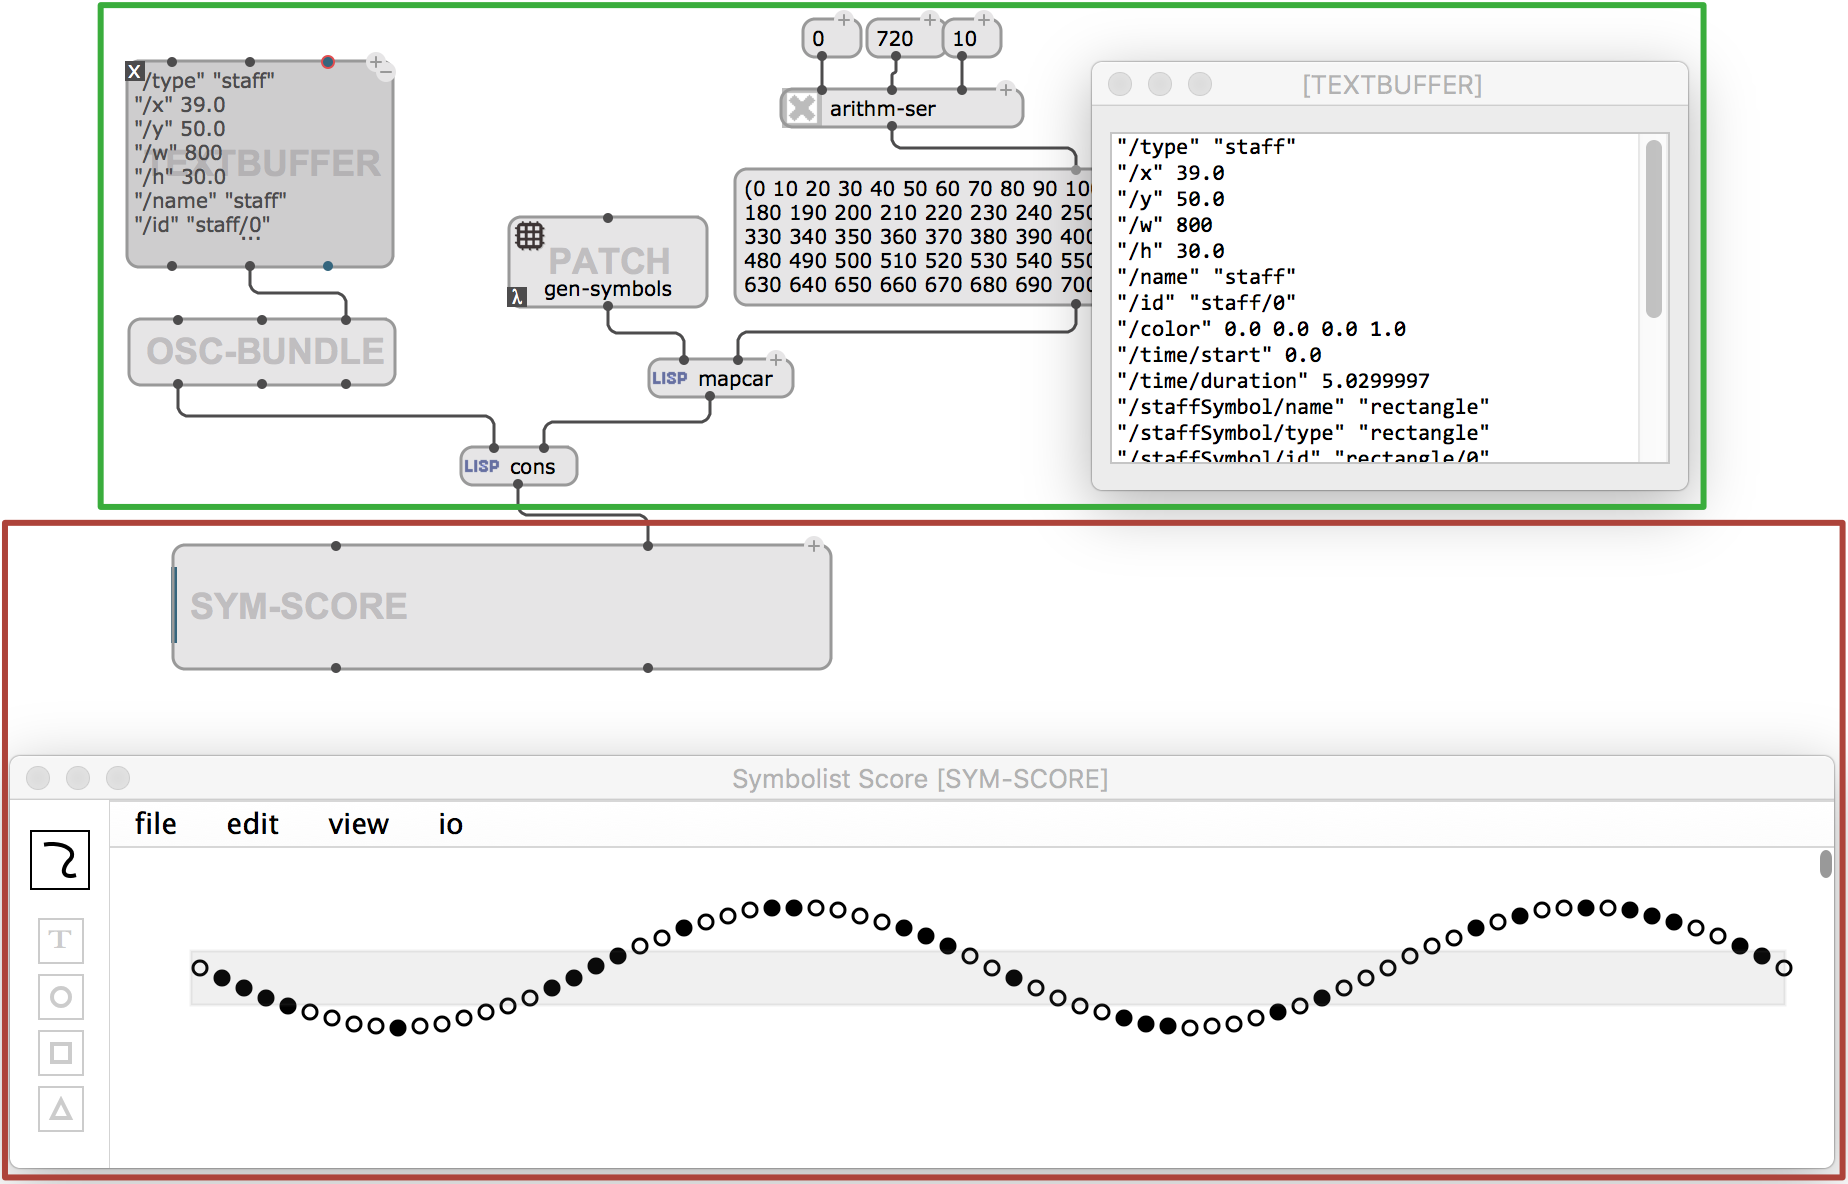
\includegraphics[keepaspectratio=true, width=\textwidth]{LeProjetSymbolist/i/symbolistOMObject.png}
	\caption{L'objet \textit{symbolist} dans OpenMusic}
	\label{fig:symbolistOMObject}
	\small
	\it
	En \textcolor{red}{rouge}, l'objet \emph{symbolist} \og sym-score \fg et l'éditeur graphique associé.
	En \textcolor{green}{vert}, les objets \emph{OpenMusic} servant à la création de bundles OSC envoyés à l'objet \emph{sym-score}.
\end{figure}

L'objet \textit{symbolist} dans sa version \textit{OpenMusic} reçoit des bundles OSC et crée les symboles correspondant dans la partition. Ensuite, le contenu de la partition peut être envoyé sur la sortie, en utilisant la barre de lecture \textit{OpenMusic} (activée par la touche espace).    

\paragraph{Fonctionnalités existantes} Afin de dresser un bilan des fonctionnalités implantées dans \textit{symbolist}, des \textit{user-stories}\footnote{Une \textit{user-story} est une manière d'exprimer une fonctionnalité logiciel, répandue chez les praticiens de la philosophie Agile. Une \textit{user story} prend la forme: \og En tant que tel type d'utilisateur, j'effectue telle action dans tel but \fg. De cette manière, une fonctionnalité est exprimée du point de vue de l'utilisateur, évitant l'écueil d'une formalisation trop technique. } ont été écrites à partir des possibilités du logiciel.
La liste des \textit{user stories} implantées dans \textit{symbolist} au début du stage est la suivante:
\begin{itemize}[label=--]
	\item En tant que compositeur, je dessine des courbes pour créer de nouveaux symboles.
	\item En tant que compositeur, je dessine des formes géométriques pour créer de nouveaux symboles.
	\item En tant que compositeur, j'écris du texte pour créer de nouveaux symboles ou pour annoter ma partition.
	\item En tant que compositeur, j'édite les propriétés d'un symbole existant pour définir sa forme.
	\item En tant que compositeur, je groupe des symboles entre eux pour créer un nouveau symbole.
	\item En tant que compositeur, je transforme un symbole en \textit{staff}, pour définir une référence temporelle dans la partition.
	\item En tant que compositeur, j'associe un symbole à un \textit{staff} pour lui procurer une valeur temporelle.
	\item En tant que compositeur, je peux ajouter un de mes propres symboles à la palette pour le réutiliser ensuite.
	\item En tant que compositeur, je peux annuler/recommencer les actions effectuées sur la partition pour la maintenir dans une état cohérent.
	\item En tant que compositeur, je peux lire le contenu de ma partition à un temps $t$. 
\end{itemize}

Les \textit{user stories} concernant le dessin sur la partition ont été réparties en catégories. En effet, chaque type de symboles est accompagné de problématiques spécifiques, ce qui fait considérer la création de texte, de courbes ou de formes prédéfinies comme des fonctionnalités à part entière.